\documentclass[sigconf]{acmart}

%% Submission version for GeoSearch 2026 (single-blind, 4 pages). The ACM
%% rights block is filled in at camera-ready time.
\setcopyright{none}
\settopmatter{printacmref=false, printfolios=true}
\renewcommand\footnotetextcopyrightpermission[1]{}
\pagestyle{plain}

\usepackage{booktabs}
\usepackage{amsmath}
\usepackage{graphicx}
\setlength{\textfloatsep}{6pt plus 1pt minus 2pt}
\setlength{\floatsep}{5pt plus 1pt minus 1pt}
\setlength{\intextsep}{5pt plus 1pt minus 1pt}
\setlength{\dbltextfloatsep}{7pt plus 1pt minus 2pt}

\acmConference[GeoSearch '26]{The 5th ACM SIGSPATIAL International Workshop on Searching and Mining Large Collections of Geospatial Data}{November 3, 2026}{Riverside, CA, USA}
\acmYear{2026}
\copyrightyear{2026}

\newcommand{\conf}{\mathcal{C}}
\newcommand{\acc}{\mathrm{acc}}

\title{Trust the View That Sees the Target: Mining Cross-View Conflicts for Reliability-Gated Disaster Damage Assessment}

\author{Yifan Yang}
\email{yyang295@tamu.edu}
\affiliation{%
  \department{Department of Geography}
  \institution{Texas A\&M University}
  \city{College Station}
  \state{Texas}
  \country{USA}
}

\author{Lei Zou}
\authornote{Corresponding author.}
\email{lzou@tamu.edu}
\affiliation{%
  \department{Department of Geography}
  \institution{Texas A\&M University}
  \city{College Station}
  \state{Texas}
  \country{USA}
}

\begin{abstract}
Paired ground-level and overhead imagery is now collected at scale after
disasters, and fusing the two views for building damage assessment is standard
practice. Fusion is almost always \emph{symmetric}: both views are trusted
equally everywhere. We mine three paired collections---inspection photographs
from the 2025 Eaton wildfire and street-view panoramas from Hurricanes Ian and
Milton, each matched to VHR overhead tiles---for \emph{conflict cases}, the
10--33\% of samples on which independently trained single-view models
disagree. On these cases an oracle that trusts the correct view exceeds every
tested fusion method by 0.37--0.41 accuracy, a gap that survives convergence,
calibration, and backbone changes. We close part of it with a
visibility-conditioned reliability gate: a linear model over
building-visibility features from a frozen segmenter, calibrated per-view
confidences, and cross-view disagreement. Under a five-seed protocol with
pooled paired tests, the gate is the only method that significantly beats
calibrated probability averaging (wildfire conflicts $+0.051$, $p=0.0001$) and
end-to-end fusion ($+0.072$ on conflicts, $p<10^{-4}$), with parity on the
panoramic datasets. A controlled field-of-view intervention shows the
mechanism is causal: cropping panoramas toward the building doubles the fusion
benefit while geometrically identical random crops do not. Finally, the
spatial density of mined conflicts predicts tile-level damage without labels
(Spearman $r=0.615$, $p=0.001$) while single-view uncertainty anti-correlates.
Conflict mining turns ``does fusion help?'' into ``which view should be
trusted, where, and why?''.
\end{abstract}

\keywords{cross-view fusion, street-view imagery, satellite imagery, disaster damage assessment, reliability estimation, GeoAI}

\begin{document}

\maketitle

\section{Introduction}
Rapid building-level damage assessment increasingly draws on two large
geospatial image collections at once. Overhead imagery gives synoptic coverage
within hours and anchors standardized damage mapping~\cite{gupta2019creating};
ground-level imagery, from crowdsourced street-view panoramas to official
inspection photographs, supplies the facade and debris evidence that overhead
sensors cannot see~\cite{zhai2020damage,yang2025hyperlocal}. Cross-view methods
that pair the two collections serve geolocalization and damage
mapping~\cite{li2025cross,yin2026triple,li2026towards}, fusion
classification~\cite{xiao2023cross}, and multimodal
arbitration~\cite{yang2026damagearbiter}, and the standard finding is
encouraging: fusion improves average accuracy over either view.

We argue that average accuracy hides both the real value and the real
limitation of cross-view fusion. Most records in a paired collection are
easy---both views agree---and fusion adds little. The operationally
interesting records are the \emph{conflicts}: samples on which independently
trained single-view models disagree. Conflicts concentrate where one sensor is
blind: a facade intact from above but gutted at street level, or a roof
destroyed above vegetation that hides it from the road. Finding these records
in a large collection, deciding which view to believe for each, and reading
their spatial distribution is a search-and-mining problem as much as a
modeling one. We therefore make conflict cases the unit of analysis and ask
three questions. \textbf{(1) How much information do fusion methods leave
unused on conflicts?} We measure an \emph{oracle single-view gap}, the margin
between an oracle that trusts whichever view is correct per sample and the
best available method; across three disasters it is 0.37--0.41 accuracy,
several times any fusion gain. \textbf{(2) Can it be recovered, and how?}
Per-sample view reliability is largely predictable from whether the ground
image actually \emph{sees the target building}; a \emph{linear} gate over
segmentation-derived visibility, calibrated confidence, and disagreement
features mixes existing predictors per sample and reads as a one-sentence
rule. \textbf{(3) Is the regime effect causal?} Datasets differ in hazard,
geography, sensors, and labels at once, so we manipulate alignment
\emph{within} a dataset with a controlled cropping intervention. A fourth
result pays off directly for mining post-disaster collections: the spatial
density of conflicts is an unsupervised damage map, computable before any
labels exist. Code, protocols,
and derived tables: \url{https://github.com/rayford295/CrossViewGate}.

\section{Data and Protocol}
We use three paired street/overhead collections spanning two hazards and,
critically, two ground-view \emph{observation regimes} (Table~\ref{tab:data}).
\textbf{Eaton wildfire (Altadena, CA):} building-level CAL~FIRE Damage
Inspection (DINS) photographs after the January 2025 fire, paired by
geolocation with post-event VHR overhead tiles; the six-level native scale is
mapped to an ordinal three-class task (no/trace, damaged--repairable,
destroyed). \textbf{Hurricane Ian:} the released CVIAN pairing from
CVDisaster~\cite{li2025cross}, Mapillary panoramas over Sanibel Island with
27~cm post-event satellite imagery and three-level damage-perception labels
(4,121 pairs as distributed). \textbf{Hurricane Milton:} a street-view/satellite
pairing over Florida after the October 2024 hurricane, constructed
analogously.

\begin{table}[t]
  \caption{Datasets. Regime describes how the ground view observes the labeled
  building; pairs are train/val/test under the headline protocol.}
  \label{tab:data}
  \centering
  \scriptsize
  \setlength{\tabcolsep}{3pt}
  \begin{tabular}{lllr}
    \toprule
    Dataset & Ground view & Regime & Pairs \\
    \midrule
    Eaton wildfire & CAL FIRE DINS photos & property-centric & 6.5k / 1,966 / 1,984 \\
    Hurricane Ian & Mapillary 360$^\circ$ panoramas & panoramic & 3,248 / 573 / 300 \\
    Hurricane Milton & 360$^\circ$ panoramas & panoramic & 1,740 / 307 / 254 \\
    \bottomrule
  \end{tabular}
\end{table}

\paragraph{Splits and leakage.}
Eaton is split by property and tile so all photographs of a structure fall in
one partition. The headline Ian numbers keep the release-derived split for
comparability with CVDisaster; an audit against the official CVIAN position
GeoJSON found that 299/300 of its test samples share a Mapillary sequence with
training data, so we also report a repaired $0.005^\circ$ spatial-block
protocol with a 25~m buffer (Section~\ref{sec:results}). The two protocols are
never mixed.

\section{Method}
\paragraph{Base models and conflict cases.}
For each dataset we train \textit{street\_only} and \textit{remote\_only}
(ResNet-18~\cite{he2016deep}, linear head), \textit{concat} (both encoders,
MLP head), and \textit{crossview} (both encoders, learned interaction head;
the end-to-end fusion reference) under one protocol: class-balanced
cross-entropy, image size 224, AdamW, up to 15 epochs with patience-4 early
stopping on validation macro-F1, five seeds; a ResNet-50/CLIP/DINOv2 sweep
confirmed no conclusion depends on the backbone. With
$s(x)$, $r(x)$ the single-view predictions, the \textbf{conflict subset} is
$\conf=\{x: s(x)\neq r(x)\}$; conflict rates are 9.6\% (Eaton), 33.2\% (Ian),
25.7\% (Milton).

\paragraph{Oracle single-view gap.}
The oracle counts a conflict sample correct if \emph{either} single view is
correct. For a method $m$ we report conflict accuracy $\acc_{\conf}(m)$ and the
\textbf{oracle-gap closure}
\begin{equation}
\mathrm{closure}(m)=
\frac{\acc_{\conf}(m)-\acc_{\conf}(\text{best single})}
     {\acc_{\conf}(\text{oracle})-\acc_{\conf}(\text{best single})}.
\label{eq:closure}
\end{equation}
The oracle uses no information beyond \emph{which} of two fixed models to
trust; it bounds arbitration between existing predictors, not new models.

\paragraph{Calibration decomposition.}
Averaging miscalibrated probabilities can win or lose for reasons unrelated to
information content~\cite{guo2017calibration}, so we fit one temperature per
view on validation predictions and re-evaluate every training-free fusion
baseline on calibrated probabilities. Scaling leaves the argmax unchanged, so
$\conf$ is identical before and after.

\paragraph{Visibility-conditioned reliability gate.}
A frozen SegFormer-B0~\cite{xie2021segformer} trained on ADE20K yields four
building-visibility features per street image: building pixel ratio, the ratio
inside a centered crop of half the image size, their difference (a centering
signal), and the normalized centroid distance from the image center. The gate's
eleven features add calibrated confidence and entropy for both views, the
confidence gap, the Jensen--Shannon divergence between the calibrated
distributions, and a disagreement flag. It outputs softmax weights over
street, remote, and crossview probabilities and is fit on the validation split
by minimizing the NLL of the gated mixture with z-scored features. The
headline gate is \emph{linear}: a small MLP matched it throughout, and linear
coefficients are directly readable. It adds one segmentation pass and a
linear fit on top of any deployed pair of models and needs only their output
probabilities.

\paragraph{Field-of-view intervention.}
Each $1024\times512$ panorama is cropped to a $256\times256$ window
(90$^\circ$ horizontal FOV, horizon band) either \textbf{building centered},
at the circular-mean azimuth of the SegFormer building mask, or
\textbf{random}, at a per-sample reproducible uniform azimuth. The variants
share size, projection, and information budget and differ only in whether the
window is aimed at the built structure. We retrain \textit{street\_only} and
\textit{crossview} on each variant (three seeds), reuse the unchanged remote
models, and compare conflict gains.

\paragraph{Conflict density.}
We average seed-wise street and remote probabilities, aggregate to geographic
tiles, and compute per tile the hard conflict density (fraction of argmax
disagreements) and a single-view uncertainty control (mean predictive
entropy), each correlated (Spearman) with the tile's mean ordinal damage.

\paragraph{Statistics.}
Instead of ``significant in $k$ of $N$ seeds'', we average each sample's
paired correctness difference over the seeds in which it qualifies (for
conflict scope, the seeds in which the single views disagree on it) and test
$\mathbb{E}[\delta]=0$ with a two-sided sign-flip permutation test (20,000
permutations) and percentile bootstrap 95\% intervals.

\begin{table*}[t]
  \caption{Test-set results (five-seed means; accuracy std $\le 0.03$
  everywhere). Conflict accuracy is computed on the per-seed conflict subset;
  closure follows Eq.~\eqref{eq:closure} with the oracle at 0.961 / 0.896 /
  0.964 conflict accuracy (gap 0.410 / 0.367 / 0.407). Gate = three-view
  linear reliability gate.}
  \label{tab:main}
  \centering
  \small
  \setlength{\tabcolsep}{5pt}
  \begin{tabular}{lccccccccc}
    \toprule
    & \multicolumn{3}{c}{Eaton wildfire (conflict rate 9.6\%)} & \multicolumn{3}{c}{Hurricane Ian (33.2\%)} & \multicolumn{3}{c}{Hurricane Milton (25.7\%)} \\
    \cmidrule(lr){2-4}\cmidrule(lr){5-7}\cmidrule(lr){8-10}
    Method & Acc. & Conflict acc. & Closure & Acc. & Conflict acc. & Closure & Acc. & Conflict acc. & Closure \\
    \midrule
    street\_only & 0.931 & 0.486 & --- & 0.703 & 0.529 & --- & 0.759 & 0.557 & --- \\
    remote\_only & 0.929 & 0.475 & --- & 0.648 & 0.367 & --- & 0.721 & 0.407 & --- \\
    concat & 0.930 & 0.674 & 0.29 & 0.709 & 0.588 & 0.15 & 0.766 & 0.622 & 0.16 \\
    crossview (end-to-end fusion) & 0.940 & 0.699 & 0.35 & \textbf{0.735} & \textbf{0.624} & \textbf{0.25} & 0.776 & \textbf{0.649} & \textbf{0.22} \\
    calibrated probability averaging & 0.954 & 0.732 & 0.44 & 0.731 & 0.617 & 0.24 & 0.776 & 0.626 & 0.17 \\
    \textbf{reliability gate (linear)} & \textbf{0.959} & \textbf{0.768} & \textbf{0.52} & 0.731 & 0.618 & 0.23 & \textbf{0.777} & 0.631 & 0.18 \\
    \bottomrule
  \end{tabular}
\end{table*}

\begin{figure*}[t]
  \centering
  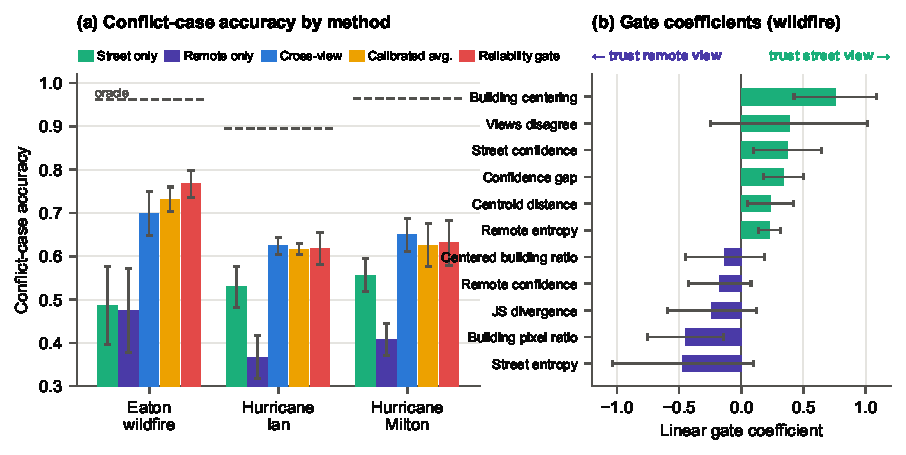
\includegraphics[width=0.62\textwidth]{../../figures/fig3_gate.pdf}
  \Description{Left: grouped bars of conflict-case accuracy for five methods on
  three datasets with the oracle as a dashed line; the gate is highest on the
  wildfire and at parity on the hurricanes. Right: linear gate coefficients on
  the wildfire; building centering, street confidence and confidence gap push
  trust toward the street view, street entropy and building pixel ratio toward
  the remote view.}
  \caption{(a) Conflict-case accuracy by method (mean $\pm$ std over five
  seeds; dashed line = oracle). (b) Linear gate coefficients on the wildfire
  (mean $\pm$ std over seeds); positive values shift trust toward the street
  view.}
  \label{fig:gate}
\end{figure*}

\section{Results}
\label{sec:results}
\paragraph{Overall and the oracle gap.}
Table~\ref{tab:main} shows three patterns. Cross-view fusion beats both single
views on conflicts on every dataset, significantly under the pooled tests
(crossview $-$ street: Eaton $+0.246$, $p<10^{-4}$; Ian $+0.078$, $p=0.013$;
Milton $+0.141$, $p=0.006$). Once single-view models are converged and
calibrated, \emph{simple probability averaging is a strong baseline}: on Eaton
it exceeds vanilla crossview (0.954 vs.\ 0.940), and end-to-end fusion does not
significantly beat it anywhere (Eaton conflicts $+0.034$, $p=0.073$); claims
that learned fusion beats simple aggregation may be artifacts of undertrained
or miscalibrated baselines, as ours were in a three-epoch pilot. And the oracle gap dwarfs all of this: knowing \emph{which existing
model to trust} per sample would add 0.37--0.41 conflict accuracy. Calibration
does not explain it---temperatures are moderate (1.0--1.75) and expected
calibration error falls from 0.02--0.14 to 0.01--0.06, yet calibrated
averaging closes at most 44\% of the gap. The unexploited information is about
\emph{when} each view is reliable.

\paragraph{The reliability gate.}
On the property-centric dataset the gate does what the mechanism predicts
(Figure~\ref{fig:gate}a): $+0.072$ conflict accuracy over end-to-end fusion
(95\% CI $[+0.046,+0.097]$, $p<10^{-4}$), $+0.018$ on the full test set
($[+0.014,+0.023]$, $p<10^{-4}$), and $+0.051$ over calibrated averaging
($[+0.026,+0.077]$, $p=0.0001$), for a 52\% closure, the only method above one
half. On the panoramic datasets, where street views rarely see the target
(mean building pixel ratio 0.027 on Ian vs.\ 0.119 on Eaton), the gate has
little visibility signal to exploit and sits at parity (vs.\ crossview: Ian
$+0.005$, $p=0.70$; Milton $-0.015$, $p=0.57$), never significantly worse. This
asymmetry \emph{is} the finding: gating pays where ground evidence is
target-aligned and degrades gracefully where it is not. The coefficients
(Figure~\ref{fig:gate}b) are stable in sign across seeds: street entropy
carries the largest negative weight; building centering and the confidence gap
are positive. The learned rule is the one an analyst would state: \emph{trust
the street view when it is confident and actually looking at the building.} A
gate fit on Ian transfers zero-shot to Eaton with 0.27 closure; visibility
features are regime-scaled, so a universal gate remains open.

\begin{table}[t]
  \caption{Field-of-view intervention (three seeds; remote models unchanged).
  Conflict gain = crossview $-$ best single view on conflicts.}
  \label{tab:fov}
  \centering
  \scriptsize
  \setlength{\tabcolsep}{4pt}
  \begin{tabular}{llccc}
    \toprule
    Dataset & Street-view variant & Street acc. & Conflict gain & Closure \\
    \midrule
    Ian    & original panorama       & 0.709 & $+0.064$ & 0.166 \\
    Ian    & building-centered crop  & 0.648 & $\mathbf{+0.109}$ & \textbf{0.269} \\
    Ian    & random crop (control)   & 0.574 & $+0.042$ & 0.072 \\
    \midrule
    Milton & original panorama       & 0.740 & $+0.067$ & 0.177 \\
    Milton & building-centered crop  & 0.693 & $\mathbf{+0.149}$ & \textbf{0.365} \\
    Milton & random crop (control)   & 0.654 & $+0.055$ & 0.128 \\
    \bottomrule
  \end{tabular}
\end{table}

\paragraph{Causal field-of-view intervention.}
Building-centered cropping raises the conflict gain on both hurricanes
(Table~\ref{tab:fov}); on Milton the closure doubles (0.177 $\to$ 0.365),
reaching two-thirds of the wildfire level, while random cropping with
identical geometry lowers it. The building-minus-random contrast is positive
in 6/6 dataset--seed pairs. Building-centered cropping \emph{lowers}
street-only accuracy (panoramic context is informative for the overall task)
yet \emph{raises} the fusion benefit: the gain comes not from a stronger street
model but from the two views attending to the same object, and the random
control rules out resolution and cropping artifacts. Street-view target
alignment is the causal variable behind the regime effect, which grounds the
gate's visibility features as causal rather than merely correlated.

\begin{figure*}[t]
  \centering
  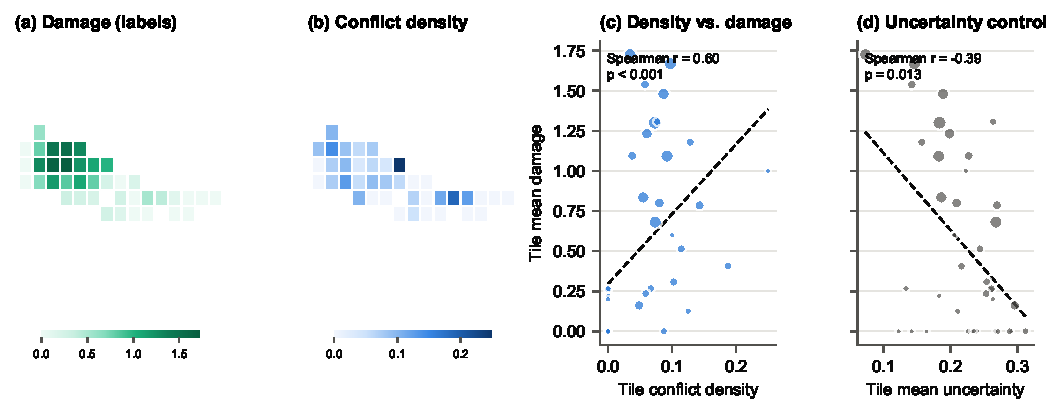
\includegraphics[width=0.62\textwidth]{../../figures/fig5_conflict_density.pdf}
  \Description{Four panels for the Eaton wildfire: a tile map of labeled
  damage, a tile map of conflict density computed without labels, a scatter of
  density against damage with positive rank correlation, and the single-view
  uncertainty control with negative correlation.}
  \caption{Conflict density as a label-free damage map (Eaton wildfire).
  (a)~Labeled tile damage. (b)~Tile conflict density computed without labels.
  (c)~Their rank correlation. (d)~The single-view uncertainty control, which
  anti-correlates with damage. Point size reflects tile sample count.}
  \label{fig:density}
\end{figure*}

\paragraph{Mining conflicts as a spatial damage signal.}
On the wildfire, hard conflict density over overhead tiles is a strong
label-free predictor of tile damage (Spearman $r=0.615$, $p=0.001$ on 25
overhead tiles; $r=0.60$, $p<0.001$ on a $0.01^\circ$ grid,
Figure~\ref{fig:density}), and it strengthened under converged models
($0.545\to0.615$). The uncertainty control fails
instructively: it \emph{anti-correlates} with damage ($r=-0.37$ to $-0.52$)
because burned-to-the-ground parcels are easy, confident classifications
(Figure~\ref{fig:density}). Conflict density is therefore not repackaged model
uncertainty but the spatial signature of two sensors disagreeing about the
world, which concentrates where damage disrupts the usual correspondence
between facade and roof evidence. Damage on Eaton is spatially autocorrelated
(Moran's $I=0.27$, $p=0.0001$), so tile correlations partly reflect spatial
structure. On Milton the signal falls below significance under converged
models ($r=0.289$) as better single-view models disagree less; the wildfire
case is the robust result.

\paragraph{External comparison and split repair.}
On the same CVIAN pairing, CVDisaster's CGCViT~\cite{li2025cross} reports
77.96 overall accuracy (street 74.50, satellite 67.07) with a 20M-parameter
encoder under a random split; our legacy-protocol ResNet-18 crossview reaches
$73.5\pm1.5$ (street 70.3, remote 64.8). Under the repaired spatial-block split
with a 25~m buffer, macro-F1 drops by 0.049--0.097 across modes: random or
index-based splits overstate spatial generalization, the single-view ranking
(street $>$ satellite) is stable, and the size of the cross-view advantage is
protocol-dependent.

\section{Discussion and Conclusion}
The 0.37--0.41 oracle gap measures the opportunity within the restricted
choice between two existing single-view models, and it dwarfs what
architectural innovation in symmetric fusion has produced. For mining paired
geospatial collections the productive question is therefore not ``how should
features be fused?'' but ``when should each view be believed?''. The gate
closes half of the gap on property-centric imagery with eleven interpretable
features; the remaining half is a quantified target for richer visibility
descriptors (occlusion, viewing distance, image quality) and pre-event
reference imagery. Operationally, the gate costs one frozen segmentation pass
per street image plus a temperature and a linear fit on validation
predictions, needs only the output probabilities of existing models, and
states its rule in one sentence, which matters where automated triage must be
auditable. Where ground imagery is panoramic and rarely target-aligned
(crowdsourced street view), calibrated averaging captures most of the
achievable benefit; where it is property-centric (inspection programs,
insurance photography), gating pays.
Because the causal driver is alignment rather than hazard, capture policy is
itself an intervention: aiming cameras at structures, or cropping panoramas
toward detected buildings, raises the value of every downstream fusion
component.

\paragraph{Limitations.}
The property-centric regime is represented by one (large) wildfire dataset;
Milton is small (2,301 pairs); the repaired CVIAN test has six spatial blocks
connected by shared Mapillary sequences, so strong spatial-generalization
claims need more independent groups; the ADE20K segmenter measures
built-structure visibility, not \emph{the} target building; the density signal
needs replication on further georeferenced disasters; and cross-disaster gate
transfer is partial.

\paragraph{Conclusion.}
Measured on the records where the views disagree, symmetric cross-view fusion
leaves 0.37--0.41 accuracy on the table across three real disasters. A linear,
interpretable, visibility-conditioned gate recovers a significant fraction of
it; a controlled field-of-view intervention shows that the mechanism,
street-view target alignment, is causal; and the disagreement signal itself,
aggregated spatially, is a label-free damage map that plain uncertainty cannot
replicate. Mining conflicts converts ``does fusion help?'' into ``which view
should be trusted, where, and why?''.

\begin{acks}
The authors used AI-based assistance for experiment automation, grammar
checking, and editorial compression, reviewed all content, and take full
responsibility for the work. Supported by the Texas A\&M University Environment
and Sustainability Initiative (ESI) through the Environment and Sustainability
Graduate Fellow Award.
\end{acks}

\bibliographystyle{ACM-Reference-Format}
\bibliography{references}

\end{document}
